\documentclass[fontsize=12pt,paper=a4,twoside]{scrartcl}

\newcommand{\grad}{\ensuremath{^{\circ}} }
\renewcommand{\strut}{\vrule width 0pt height5mm depth2mm}

\usepackage[utf8]{inputenc}
\usepackage[final]{pdfpages}
% obere Seitenränder gestalten können
\usepackage{fancyhdr}
\usepackage{moreverb}
% Graphiken als jpg, png etc. einbinden können
\usepackage{graphicx}
%\usepackage{stmaryrd}
% Floats Objekte mit [H] festsetzen
\usepackage{float}
% setzt URLs schön mit \url{http://bla.laber.com/~mypage}
\usepackage{url}
% Externe PDF's einbinden können
\usepackage{pdflscape}
% Verweise innerhalb des Dokuments schick mit " ... auf Seite ... "
% automatisch versehen. Dazu \vref{labelname} benutzen
\usepackage[ngerman]{varioref}
\usepackage[ngerman]{babel}
\usepackage{ngerman}
% Bibliographie
\usepackage{bibgerm}
% Tabellen
\usepackage{tabularx}
\usepackage{supertabular}
\usepackage[colorlinks=true, pdfstartview=FitV, linkcolor=blue,
            citecolor=blue, urlcolor=blue, hyperfigures=true,
            pdftex=true]{hyperref}
\usepackage{bookmark}

\newboolean{langversion} %Deklaration
\setboolean{langversion}{true} %Zuweisung ist 'false' für Blockkurs
\newcommand{\highlight}[1]{\textcolor{blue}{\textbf{#1}}}
\newcommand{\nurlangversion}[0]{%
\ifthenelse{\boolean{langversion}}{\highlight{}}{\highlight{Entfällt in SWP-1}}}

\newcommand{\swp}[0]{\ifthenelse{\boolean{langversion}}%
{Software--Projekt 2}{Software--Projekt 1}}
\newcommand{\jahr}[0]{2014}
\newcommand{\semester}[0]{\ifthenelse{\boolean{langversion}}{SoSe}{SoSe} \jahr}

% Damit Latex nicht zu lange Zeilen produziert:
\sloppy
%Uneinheitlicher unterer Seitenrand:
%\raggedbottom

% Kein Erstzeileneinzug beim Absatzanfang
% Sieht aber nur gut aus, wenn man zwischen Absätzen viel Platz einbaut
\setlength{\parindent}{0ex}

% Abstand zwischen zwei Absätzen
\setlength{\parskip}{1ex}

% Seitenränder für Korrekturen verändern
\addtolength{\evensidemargin}{-1cm}
\addtolength{\oddsidemargin}{1cm}

\bibliographystyle{gerapali}

% Lustige Header auf den Seiten
  \pagestyle{fancy}
  \setlength{\headheight}{70.55003pt}
  \fancyhead{}
  \fancyhead[LO,RE]{\swp\\ \semester{}
  \\Anforderungsspezifikation}
  \fancyhead[LE,RO]{Seite \thepage\\\slshape \leftmark\\\slshape \rightmark}

%
% Und jetzt geht das Dokument los....
%

\begin{document}

% Lustige Header nur auf dieser Seite
  \thispagestyle{fancy}
  \fancyhead[LO,RE]{ }
  \fancyhead[LE,RO]{Universität Bremen\\FB 3 -- Informatik\\
  Dr. Karsten Hölscher \\Tutor: Karsten Hölscher}
  \fancyfoot[C]{}

% Start Titelseite
  \vspace{3cm}

  \begin{minipage}[H]{\textwidth}
  \begin{center}
  \bf
  \Large
  \swp{} \jahr\\
  \smallskip
  \small
  VAK 03-BA-901.02\\
  \vspace{3cm}
  \end{center}
  \end{minipage}
  \begin{minipage}[H]{\textwidth}
  \begin{center}
  \vspace{1cm}
  \bf
  {\Large Anforderungsspezifikation}\\
  \vspace{3ex}
  $<$Name der Projektgruppe$>$\\% Ersetzen
  \vfill
  \end{center}
  \end{minipage}
  \vfill
  \begin{minipage}[H]{\textwidth}
  \begin{center}
  \sf
  \begin{tabular}{lrr}
  Patrick Hollatz & phollatz@tzi.de & 2596537 \\
  Tobias Dellert & tode@tzi.de & 2936941 \\
  Tim Ellhoff & tellhoff@tzi.de & 2520913\\
  Daniel Pupat & dpupat@tzi.de & 2703053 \\
  Olga Miloevich & halfelv@tzi.de  & 2586817\\  
  Tim Wiechers & tim3@tzi.de & 2925222 \\
  \end{tabular}
  \\ ~
  \vspace{2cm}
  \\
  \it Abgabe: TT. Monat JJJJ --- Version 1.1\\ ~
  \end{center}
  \end{minipage}

% Ende Titelseite

% Start Leerseite

\newpage

  \thispagestyle{fancy}
  \fancyhead{}
  \fancyhead[LO,RE]{\swp{}\\ \semester{}
  \\Anforderungsspezifikation}
  \fancyhead[LE,RO]{Seite \thepage\\\slshape \leftmark\\~}
  \fancyfoot{}
  \renewcommand{\headrulewidth}{0.4pt}
  \tableofcontents

\newpage

  \fancyhead[LE,RO]{Seite \thepage\\\slshape \leftmark\\\slshape \rightmark}


%%%%%%%%%%%%%%%%%%%%%%%%%%%%%%%%%%%%%%%%%%%%%%%%%%%%%%%%%%%%%%%%%%%%%%%%
\section*{Version und Änderungsgeschichte}

{\em Die aktuelle Versionsnummer des Dokumentes sollte eindeutig und gut zu
identifizieren sein, hier und optimalerweise auf dem Titelblatt.}

\begin{tabular}{ccl}
Version & Datum & Änderungen \\
\hline
1.0 & 21.05.2014 & Analyse ähnlicher Systeme. \\
1.1 & TT.MM.JJJJ & .... 
\end{tabular}


%%%%%%%%%%%%%%%%%%%%%%%%%%%%%%%%%%%%%%%%%%%%%%%%%%%%%%%%%%%%%%%%%%%%%%%%
\section{Einleitung}
\nurlangversion

{\em Dieses Dokument dient als Vorlage für Eure
  Anforderungsspezifikation. Die Gliederung dieses
  Dokuments ist an die Struktur des IEEE-Standards 830.1998 angelehnt,
  weicht jedoch an einigen Stellen davon ab. Die Abweichungen sind
  im weiteren Verlauf dieses Dokuments dokumentiert. Weitere detaillierte
  Hinweise finden sich im IEEE-Standard 830.1998, der in Stud.IP      
  beziehungsweise über die Uni-Bibliothek in digitaler Form verfügbar ist
  \footnote{Bei \url{http://ieeexplore.ieee.org} im Suchfeld 'IEEE std    
   830-1998' eingeben. Funktioniert nur innerhalb des Uni-Netzes.}.}

\subsection{Zweck}
\nurlangversion

  {\em Was ist der Zweck dieser Anforderungsspezifikation? Wer sind
  die LeserInnen?}

\subsection{Rahmen}
\nurlangversion

  {\em Dieser Abschnitt soll einen groben Überblick über die zu
  erstellende Software geben: Welche Produkte sind zu erstellen (mit
  Namen)? Was tut die Software? Auch: Was tut sie nicht? Wozu soll die
  Software verwendet werden?  (Ziele etc.)}

\subsection{Definitionen, Akronyme und Abkürzungen}
\nurlangversion

  {\em Hier geht es vor allem um Begriffe aus der Anwendungsdomäne,
  d.h.\ aus der Welt des Kunden. Aber auch Begriffe, die dem Kunden
  evtl.\ fremd oder unklar sind, sollten erläutert werden.}


\subsection{Referenzen}
  {\em Neben sonstigen Quellen, die Ihr verwendet habt, können dies
  z.B.\ das Skript, dieses Beispieldokument, der zugrunde
  liegende IEEE-Standard und anderes sein}
  

\subsection{Übersicht über das Dokument}
\nurlangversion

  {\em Was enthält die Anforderungsspezifikation? Wie ist das Dokument
  organisiert?}


\section{Allgemeine Beschreibung}
\label{ch:AllgemeineBeschreibung}

\subsection{Ergebnisse der Ist-Analyse}
\nurlangversion

  {\em Hier sollten die Ergebnisse Eurer Ist-Analyse kurz
  zusammengefasst werden. Diese Beschreibung ist hilfreich, um die
  Motivation für die Anforderungen zu verstehen und um sie später
  nachzuvollziehen (z.B.\ dann wenn Anforderungen überarbeitet werden
  sollen, weil sich ihre Rahmenbedingungen geändert haben).
  
  Mögliche Inhalte: 
  \begin{itemize}
    \item Interview/Beobachtung des Kunden oder der Benutzer
    \item Analyse des bisherigen Systems und dessen Probleme 
    \item Analyse ähnlicher Systeme
    \item Auswertung der Benutzerbefragung
    \item Wie sollen die identifizierten Probleme vom neuen System adressiert werden?
  \end{itemize}
  
  N.B.: Dieser Abschnitt ist im IEEE-Standard nicht vorgesehen, aber dennoch
  sinnvoll.}
  


\subsubsection{Erstes Kundengespräch vom TT.MM.JJJJ}
\nurlangversion

\subsubsection{Interview mit einem Mitarbeiter der ...}
\nurlangversion

{\em Falls durchgeführt}

\subsubsection{Analyse eines ähnlichem Systems}

Als System haben wir uns die App Quizduell ausgesucht. Die App ist im App-Store kostenlos zu erhalten. Wir benutzen hierzu nicht die Premium-Version, da die kostenlose unserem System am nächsten kommt. Wir haben nicht die Rechte eines Administrators, weshalb sich die Analyse nur auf die App bezieht. Die App kann nur verwendet werden, wenn man eine bestehende Internet Verbindung hat.\\

\begin{figure}[H]
\centering

\includegraphics[scale=0.5]{Bilder/lade.png}
\caption{Ladebildschirm}
\end{figure}

Dies ist der Ladebildschirm, sobald die App gestartet wird.

\begin{figure}[H]
\centering
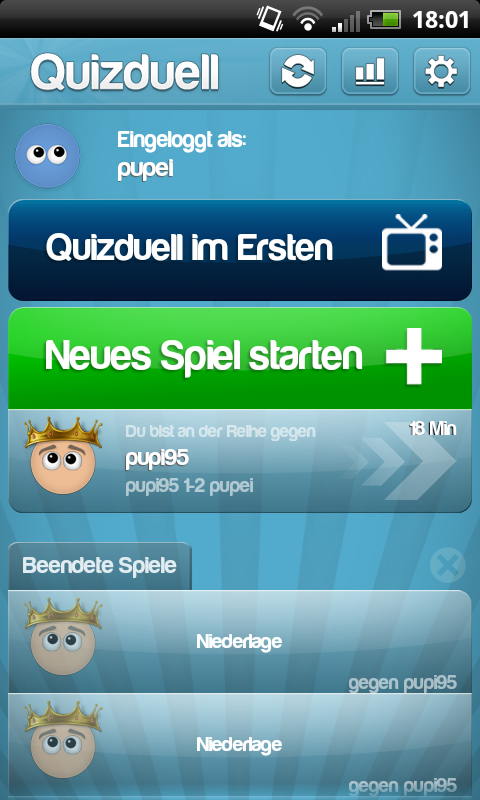
\includegraphics[scale=0.5]{Bilder/start.png}
\caption{Startbildschirm}
\end{figure}

Hier ist der Startbildschirm, nachdem man eingeloggt ist. Oben hat man die Funktionen Aktualisieren, Statistiken und Einstellungen. Beim aktualisieren wird die Seite aktualisiert. \\

\begin{figure}[H]
\centering
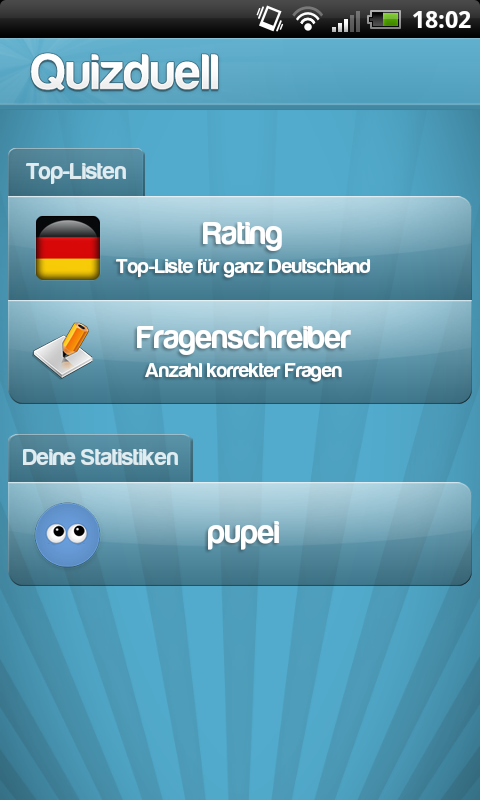
\includegraphics[scale=0.5]{Bilder/stat.png}
\caption{Statistiken}
\end{figure}

Hier kann man die Rating Liste aller Nutzer in Deutschland im Bezug auf der Punktzahl und der Anzahl der geschrieben und angenommenen Fragen sehen. Für die eigene Statistik wird eine Premium-Version benötigt.\\

\begin{figure}[H]
\centering
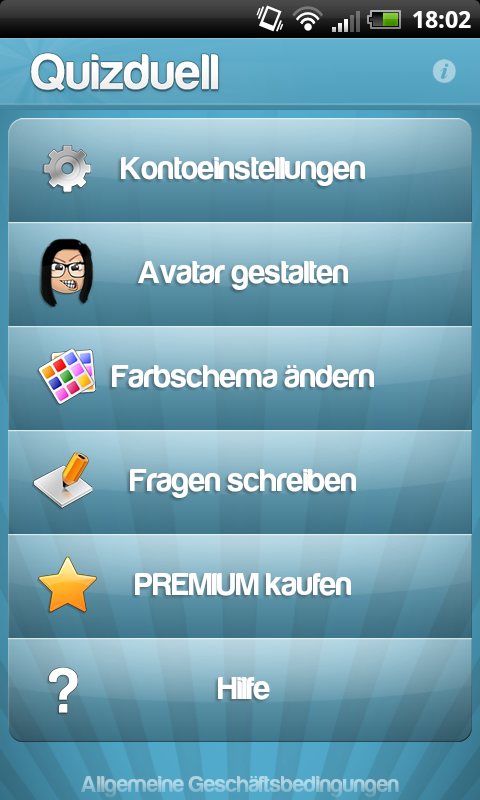
\includegraphics[scale=0.5]{Bilder/optionen.png}
\caption{Einstellungen}
\end{figure}

Unter Einstellungen kann man seine Kontoeinstellungen bearbeiten, wo man den Benutzernamen und Passwort ändern kann. Für Avatar gestalten und Farbschema ändern beötigt man die Premium-Version, welche man unter PREMIUM kaufen erwerben kann. Bei Fragen schreiben, kann man eigene Fragen schreiben, die evtl. dann übernommen werden. Bei Hilfe werden bestimmte Fragen im Hinblick auf die Benutzung beantwortet.\\

\begin{figure}[H]
\centering
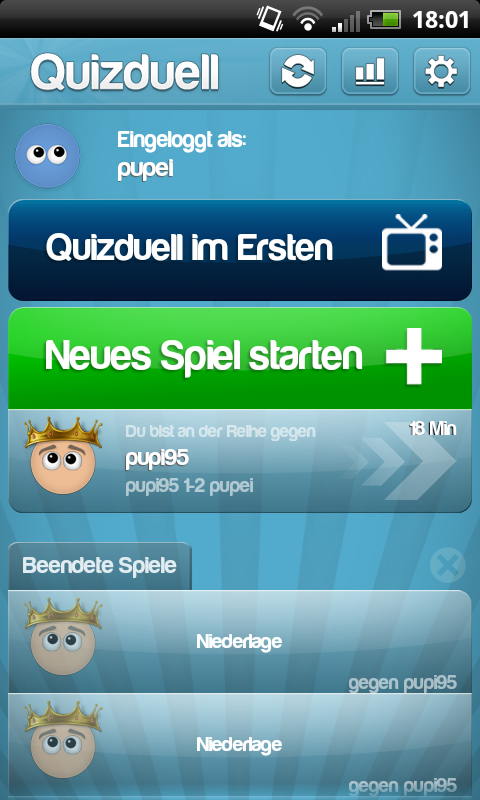
\includegraphics[scale=0.5]{Bilder/start.png}
\caption{Startbildschirm}
\end{figure}

Weiter Funktionen beim Startbildschirm sind Neues Spiel starten oder ein bereits angefangenes Spiel weiterspielen.\\

\begin{figure}[H]
\centering
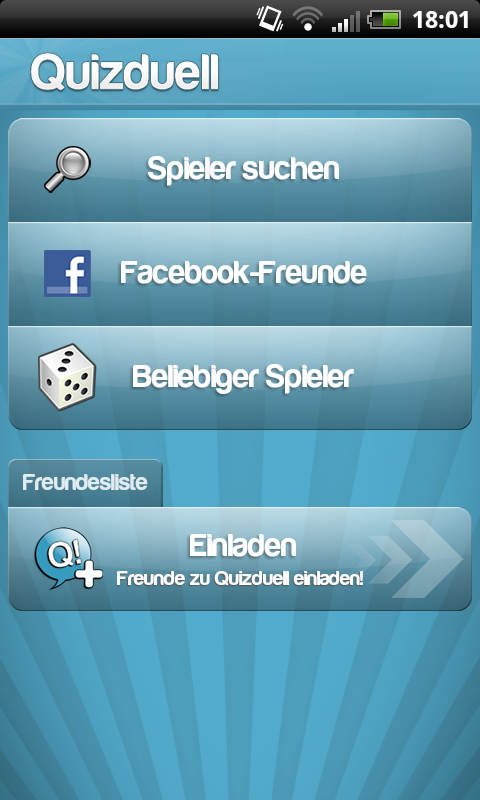
\includegraphics[scale=0.5]{Bilder/neuesspiel.png}
\caption{Bildschirm wenn man ein neues Spiel starten möchte}
\end{figure}

Wenn man ein neues Spiel starten möchte, kann man einen neuen Spieler suchen, unter Facebook Freunden suchen, falls man unter Facebook eingeloggt ist, oder gegen einen beliebigen Spieler spielen, der ebenfalls einen gesucht hat. 


\begin{figure}[H]
\centering
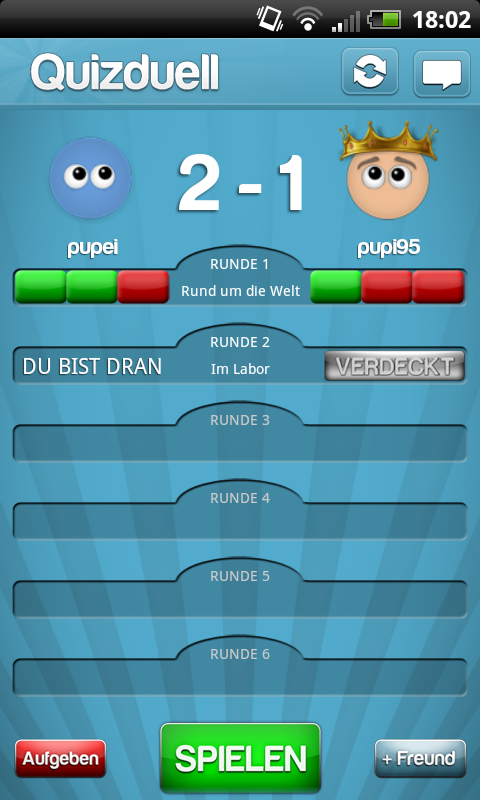
\includegraphics[scale=0.5]{Bilder/spiel.png}
\caption{Bildschirm beim neuen oder laufenden Spiel}
\end{figure}

Hier wird der bisherige Spielstand angezeigt. Insgesamt gibt es 6 Fragen, welche jeder beantworten muss. Die Spieler erhalten jeweils die gleichen Fragen. Es werden immer 2 Fragen abwechselnd gestellt, wobei der Spieler einmal eine Kategorie auswählen darf und einmal die Fragen der Kategorie des Gegners beantworten muss. Die Spieler haben 48 Stunden Zeit die Fragen zu beantworten bis das Spiel automatisch, mit einer Niederlage des Spielers der nicht geantwortet hat, endet. 

\begin{figure}[H]
\centering
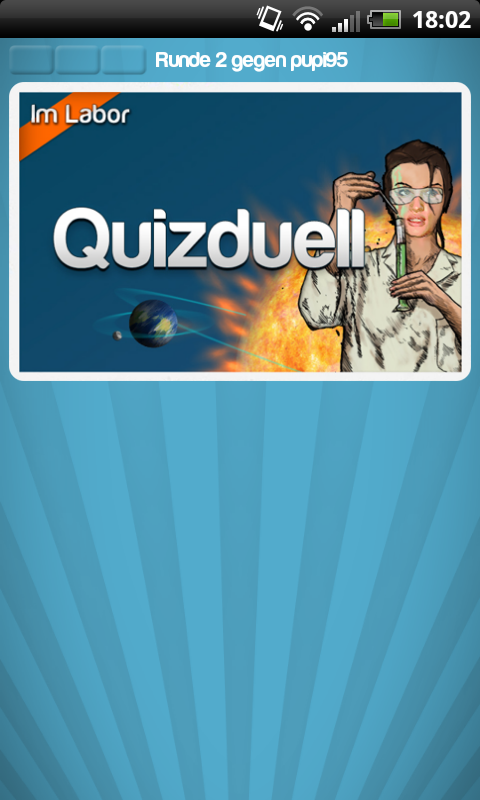
\includegraphics[scale=0.5]{Bilder/spielstart.png}
\caption{Beim Starten der Fragen}
\end{figure}

Beim Starten einer Frage erscheint erst nur eine Karte mit der Kategorie, bei einer Berührung wird die Karte umgedreht.\\

\begin{figure}[H]
\centering
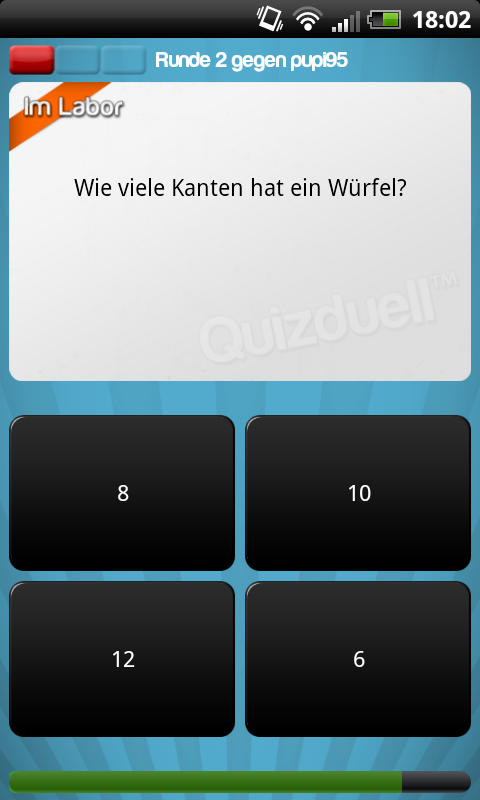
\includegraphics[scale=0.5]{Bilder/frage.png}
\caption{Anzeigen der Frage}
\end{figure}

Nun wird die Frage angezeigt, man hat 20 Sekunden Zeit um die Frage zu beantworten, sonst wird diese als Falsch gewertet.\\

\begin{figure}[H]
\centering
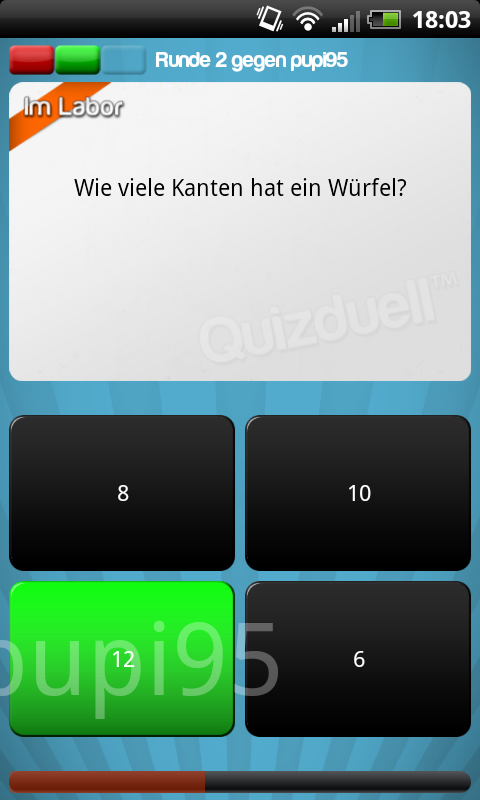
\includegraphics[scale=0.5]{Bilder/antwort.png}
\caption{Reaktion bei richtiger Antwort}
\end{figure}

Bei einer richtigen Antwort wird diese mit Grün unterlegt und Zeitgleich wird der Name des Gegners auf seiner Antort angezeigt, wenn er diese bereits beantwortet hat. Bei einer falschen wird die Antwort mit Rot unterlegt.\\

Fazit:\\
Die Quizduell App ist ein gutes System mit welcher man unseres später Vergleichen kann. Es hat viele Funktion, wie gezeigt, welche unser System ebenfalls haben muss. Es gibt allerdings auch Unterschiede, in unsere App wird es nur 3 Runden pro Runde geben und es werden keine eigenen Fragen geschrieben, außerdem wird es keine Premium-Version geben. Zudem werden wir auch eine offline-Funktion einbauen, in welcher der Spieler alleine spielen kann.\\ 

\subsection{Produktperspektive}
\nurlangversion
  
\subsubsection{Systemschnittstellen}
\nurlangversion

  {\em Schnittstellen zu anderen Systemen, z.B.\ Datenimport/-export,
  Konfigurationsdateien, anzubindende externe Dienste und deren Schnittstelle,
  Anbieten der eigenen Funktionalität als API o.ä.}
  

\subsubsection{Benutzerschnittstelle}
\nurlangversion

  {\em GUI-Design-Richtlinien und Interaktionsmechanismen (nicht
  Screenshots aller Dialoge --- die werden in Kapitel 3 gezeigt --- aber
  evtl.\ ein Screenshot, der einen groben Überblick und Eindruck des
  GUI-Designs gibt).}


\subsubsection{Hardwareschnittstellen}
\nurlangversion

  {\em Schnittstellen zu vorgegebenen Hardwarekomponenten (Name,
  Version).}
 

\subsubsection{Softwareschnittstellen}
\nurlangversion

{\em Softwarebibliotheken und --rahmenwerke (Frameworks), die benutzt
  werden sollen, mit Versionsnummer, Hersteller, Quelle etc. Dazu
  gehört auf jeden Fall Java.}

  \begin{tabular}{|l|l|l|l|}\hline
    \textbf{Name} & \textbf{Version} & \textbf{Hersteller} & \textbf{Quelle} \\\hline
    Java Runtime & 6 Update 37 & Oracle & \url{http://java.com} \\\hline
    Hibernate & 4.3.0.Beta1 Release& JBoss Community &  
   \url{http://www.hibernate.org/}\\\hline
    \ldots & & & \\\hline
  \end{tabular}

\subsubsection{Kommunikationsschnittstellen}
\nurlangversion

{\em Anforderungen an und Bandbreite von Kommunikationsnetzwerken, öffentliche
  oder auch private IP-Adressen?}

\subsubsection{Speicherbeschränkung}
\nurlangversion

  {\em min./max.\ verfügbarer Hauptspeicher und Festplattenplatz, knappe Begründung wie Ihr zu
der hier angegebenen Einschätzung gekommen seid}

\subsubsection{Operationen (Betriebsmodi)}
\nurlangversion

  {\em Welche Betriebsmodi gibt es? Warum? Welche Benutzerklasse darf
  was in welchem Betriebsmodus (Rechte)? Was ist der Zusammenhang
  zwischen Betriebsmodus und Sicherung/Wiederherstellung von Daten?}

\subsubsection{Möglichkeiten der lokalen Anpassung}
\nurlangversion

  {\em Was kann bei Auslieferung des Systems alles konfiguriert
  werden? Z.B. Pfade, Datenbankname, Server-IP usw. Hier ist nicht
  Internationalisierung gemeint!}


\subsection{Anwendungsfälle}
  {\em Auflistung und kurze Beschreibung aller relevanten
  Anwendungsfälle. Dies soll einen Überblick über alle Anwendungsfälle
  geben, die in 3.2 detailliert beschrieben werden.}


\subsection{Charakteristika der Benutzer}
  {\em Beschreibt hier Eure typischen Benutzer. Benutzt dazu die in
  der Vorlesung vorgestellten Personas. Zur Erinnerung: Ihr beschreibt
  konkrete Personen, die Repräsentanten der verschiedenen
  Benutzertypen sind (mit Name, evtl. Wohnort, Tätigkeit, Alter, Bild,
  \ldots). Diese sollten eine gewisse Motivation haben, bestimmte
  Anwendungsfälle durchzuführen (und dort auch eingesetzt werden!).}


\subsection{Einschränkungen}
\label{sec:Einschraenkungen}
{\em Dieser Abschnitt gibt einen groben Überblick über alles, was den
  Entwurf einschränken könnte. Details folgen dann in
  Abschnitt~\ref{ch:DetaillierteBeschreibung} (\glqq Detaillierte
  Beschreibung\grqq). Allgemeine Sicherheitsanforderungen könnten also
  hier kurz beschrieben werden, Details dann im
  Abschnitt~\ref{sec:softwaresystemattribute} zu Systemattributen.

  Beispiele für mögliche Einschränkungen könnten sein (die Liste ist
  nicht vollständig und nicht alle dieser Punkte sind in jedem
  möglichen Projekt relevant):

  \begin{itemize}
   \item feste Vorgaben (z.B. Policies)
   \item gesetzliche Rahmenbedingungen (z.B. Datenschutzaspekte)
   \item Hardwarebeschränkungen
   \item festgelegte Schnittstellen zu anderen Anwendungen
   \item parallele Operationen (z.B. Multithreading)
   \item zu unterstützende Prüffunktionen (auch: Audit-Funktionen;
     z.B. \glqq alle Buchungen im System müssen protokolliert und von
     einem Wirtschaftsprüfer nachvollziehbar sein\grqq)
   \item Steuerungsfunktionen (z.B. \glqq Das System kann von einem
     Techniker von Ferne gewartet werden\grqq)
   \item Anforderungen an die zu verwendende Programmiersprache
   \item Verlässlichkeit; die Verfügbarkeit eines technischen Systems 
       ist die Wahrscheinlichkeit oder das Maß, dass das System 
       bestimmte Anforderungen innerhalb eines vereinbarten
       Zeitrahmens erfüllt. Eine Beispielanforderung könnte sein, dass
       das System an jedem Tag der Woche 24 h lang in Betrieb sein 
       muss und im Jahr höchstens 2 Tage nicht verfügbar sein darf.
   \item Zuverlässigkeit; Software-Zuverlässigkeit wird definiert 
      als die Wahrscheinlichkeit einer fehlerfreien Software-Anwendung 
      über eine spezifizierte Zeitdauer und unter spezifizierten
      Umgebungsbedingungen. Hier könnte zum Beispiel eine zu
      erreichende Testabdeckung in Bezug auf ein Abdeckungsmaß
      gefordert werden: \glqq 90\,\% Anweisungsabdeckung bei den
      Komponententests\grqq.
   \item Kritikalität (Gefährlichkeit eines Versagens) der Anwendung
   \item Sicherheit
  \end{itemize}

}

\subsubsection{Rahmenbedingungen}
\nurlangversion

\subsubsection{Gesetzliche Rahmenbedingungen}
\nurlangversion
 
\subsubsection{Sicherheitskritische Aspekte}
\nurlangversion

\subsection{Annahmen und Abhängigkeiten}
\nurlangversion

  {\em Faktoren, deren Änderung zwangsläufig zu Änderungen an der
  Anforderungsspezifikation führen würde.}



\subsection{Ausblick}
\nurlangversion

  {\em Beschreibt hier knapp, welche Änderungen und Erweiterungen
  zukünftig (d.h.\ nach Auslieferung des Systems) zu erwarten sind.
  Diese Information ist wichtig für den Entwurf, um mögliche
  Änderungen frühzeitig im ersten Entwurf berücksichtigen zu können.
  Der Entwurf kann dann so gestaltet werden, dass die zukünftigen
  Anforderungen leicht realisierbar sind. Die zukünftigen
  Anforderungen sollten realistisch sein, ansonsten könnte ein unnötig
  allgemeiner und damit zu komplizierter Entwurf die Folge sein.  Auch
  dieser Abschnitt ist im IEEE-Standard nicht vorgesehen -- zumindest
  nicht explizit in Form eines eigenständigen Abschnitts. Dennoch
  handelt es sich um wertvolle Information, von der der Entwurf
  profitieren kann.}
  

\section{Detaillierte Beschreibung}
\label{ch:DetaillierteBeschreibung}
{\em Die externen Schnittstellen werden grob in Abschnitt 2
  beschrieben.  Wenn die grobe Beschreibung dort nicht genügt, kann
  sie hier detaillierter ausgeführt werden (wie vom IEEE-Standard
  vorgesehen).}

\subsection{Datenmodell}
  {\em Das Datenmodell im Kontext des Pflichtenhefts ist {\glqq}die
  Darstellung von Informationen und deren Beziehungen in einem
  fachlogischen Konzept{\grqq}. Es soll hier gezeigt werden, welche
  Einheiten für das existierende System relevant sind und welche
  Beziehungen zwischen diesen Einheiten gelten. Es handelt sich
  hierbei noch nicht um ein Datenbankschema oder eine Spezifikation
  von Klassen für die Implementierung (Entwurf), sondern um die
  Modellierung der realen Welt. Das Datenmodell ist leitend für den
  Entwurf (weil alles darin beschrieben sich auch in der Software 
  wiederfinden wird), aber nimmt den Entwurf nicht schon vorweg.
  
  Das Datenmodell soll als UML-Klassendiagramm angegeben werden.
  Wichtig ist hierbei die korrekte Verwendung der UML: Klassen,
  Attribute, Generalisierung, Assoziation, Aggregation, Komposition,
  Multiplizitäten. Außerdem sollte das Diagramm sinnvoll und gut
  lesbar sein. Dazu gehört weiterhin eine kurze Beschreibung des
  Modells mit ergänzenden Informationen, insbesondere wenn die
  Relationen durch ihren Namen nicht selbsterklärend sind. Gebt
  unbedingt ein Mengengerüst für die Daten an: Wie viele Instanzen der
  wichtigsten Klassen werden erwartet? Erwartet Ihr Änderungen im
  Datenvolumen in der Zukunft?}


\subsection{Anwendungsfälle}
  {\em Dieser Teil enthält die \textbf{funktionalen Anforderungen} an
  das System. Diese werden durch Anwendungsfälle beschrieben. Insofern
  müssen die Anwendungsfälle die Funktionalität des Systems
  vollständig abdecken. Daher müssen auch Varianten von
  Standard\-ab\-läufen sowie das Verhalten im Fehlerfall behandelt werden.
  
  In den Anwendungsfällen beschreibt Ihr, wie Eure Personas mit dem
  System interagieren, wenn sie ein bestimmtes Ziel erreichen wollen.
  Dabei sollte der Anwendungsfall zum Profil der Persona passen, also
  eine typische Anwendung seiner Personengruppe sein. Ihr solltet die
  Anwendungsfälle textuell beschreiben (im unten aufgeführten Schema)
  und im Fall von komplexen Anwendungsfällen zusätzlich
  Sequenzdiagramme verwenden, um durch graphische Darstellung das
  Verständnis zu erleichtern.  Stellt sicher, dass die
  Mindestanforderungen auf jeden Fall erfasst sind.  Weiterhin sollen
  hier noch keine Implementierungsdetails festgelegt werden, um keine
  Entwurfsentscheidungen vorwegzunehmen.

  Verwendet die Screenshots oder digitalisierten Bilder Eures
  Papierprototypen, um die Benutzungsführung in den Anwendungsfällen
  zu illustrieren und die konkrete Benutzer\-oberfläche, die es zu
  implementieren gilt, zu spezifizieren. Die Bilder sollten im Text an
  der entsprechenden Stelle referenziert werden, um das Verständnis
  für die Abläufe zu gewährleisten. Die Beschreibung muss so genau
  sein, dass klar ist, wie welche Aktionen ausgelöst werden und was
  das für Folgen hat (Beispiel: {\glqq}Benutzer startet die
  Suche{\grqq} -- wie macht er das?  {\glqq}{\ldots}durch Drücken des
  Buttons {\glq}Suche{\grq}{\grqq}). Die Spezifikation, die die
  Navigation zwischen Screens und Dialogen beschreibt, nennt man
  das Navigationsmodell. Es kann zum Beispiel in der Notation eines   
  UML-Zustandsdiagrammes ausgedrückt werden, wobei jeder Screen/Dialog als
  Zustand aufgefasst wird, Benutzerinteraktionen und sonstige Ereignisse
  als Transitionen dargestellt werden.

  Die Struktur der textuellen Beschreibung sollte sein:
  \begin{enumerate}
    \item eindeutiger Name des Anwendungsfalls mit eindeutiger Nummer
    
    \item Akteure: welche externen Instanzen interagieren mit
    dem System in diesem Anwendungsfall?  
    
    \item Vorbedingungen: Ausgangszustand, der vor Beginn des
    Anwendungsfalls gelten muss -- hier sollte auch das Ziel des Akteurs
    genannt werden
    
    \item Regulärer Ablauf: Abfolge von Aktionen der Akteure und
    Reaktionen des Systems
    
    \item Varianten: mögliche Abweichungen vom regulären Ablauf, z.B.\ 
    Auslassen oder Wiederholen von Aktionen
    
    \item Nachbedingung: Endzustand und dann mögliche Folgeaktionen 
  
    \item Fehler-/Ausnahmefälle mit deren Nachbedingung; z.B.\ wie wird
    auf ungültige Eingaben reagiert?
  \end{enumerate}
  }

\subsection{Aktionen}
  {\em Hier sollten die gleichen Aktionen wie in den Anwendungsfällen
  genannt und genauer beschrieben werden. Mit anderen Worten: Die
  Anwendungsfälle müssen vollständig durch Ausführung von Aktionen aus
  dieser Liste durchführbar sein. Im Prinzip muss es z.B.\ für jeden
  Button/Menüpunkt/Link eine Aktion geben. Dabei ist zu beachten:
  \begin{itemize}
    \item Die Namen sollten sinnvoll und eindeutig sein.

    \item Die Parameter der Aktionen sollen angegeben werden. Hier
    sollen sprechende Namen verwendet werden. Eventuell müssen die
    Parameter auch genauer erläutert werden.

    \item Es müssen maximale Ausführungszeiten für jede Operation
    angegeben werden.
    
  \item Die Gruppierung und Sortierung sollte sinnvoll sein
    (z.B. alphabetisch).
  \end{itemize}

  Wenn Ihr z.B.\ irgendwo in Eurer GUI ein Suchfeld habt, in das Ihr
  den Namen eines Kunden eintragen könnt, und einen Button, welcher die
  Suche startet, dann wird es vermutlich eine Aktion {\bf Kunde
    suchen(name)} geben. Dies ist eine Funktion, die Euer System
  bereitstellt und die durch Anklicken des Buttons ausgelöst wird. Der
  Anwendungsfall {\bf Kunde suchen} verwendet dann diese Aktion,
  enthält aber zusätzlich die Beschreibung der Interaktion mit dem
  System.
  
  Dieser Abschnitt ist im Standard im Prinzip vorgesehen, weil hierzu
  grundsätzlich eine Aussage gemacht werden muss. Die Aktionen sind
  letztlich die Produktfunktionen, während die Anwendungsfälle die
  Interaktion zwischen Akteuren und System beschreiben. }

  
\subsection{Entwurfseinschränkungen}
\nurlangversion

{\em Wurde bereits in \ref{sec:Einschraenkungen} behandelt und muss
  daher hier nicht wiederholt werden. Falls aber eine detailliertere
  Beschreibung notwendig wäre, wäre hier der geeignete Ort.}
  

\subsection{Softwaresystemattribute}
\label{sec:softwaresystemattribute}

  {\em Hier werden die sogenannten „nichtfunktionalen Anforderungen“
  spezifiziert. Dazu gehören beispielsweise:
  \begin{itemize}
    \item Performanz
    \item Zuverlässigkeit (Korrektheit, Robustheit, Ausfallsicherheit)
    \item Verfügbarkeit
    \item Sicherheit
    \item Wartbarkeit
    \item Portabilität
  \end{itemize}
}

{\em Die spezifizierten Systemattribute müssen hinreichend konkret und
  überprüfbar formuliert werden.}



\subsection{Weitere Anforderungen}
\nurlangversion

{\em In diesem Abschnitt können weitere relevante Anforderungen
  beschrieben werden, die in keine der oben genannten Abschnitte
  passen.}

\section{Anhang}
\nurlangversion

{\em Hier können weitere detailliertere Ergebnisse aus der Ist-Analyse
  oder andere Informationen, die zur Erstellung der Spezifikation
  gedient haben (z.B. Papierprototypen), angefügt werden.}

\end{document}
